\documentclass[12pt]{article}

\usepackage{sbc-template}
\usepackage{graphicx,url}
\usepackage[utf8]{inputenc}
%\usepackage[brazil]{babel}
\usepackage{xcolor}
%\usepackage[latin1]{inputenc}  


\sloppy

\title{Intelligent Classification of Legislative Propositions}

\author{Luca Peres Quinta da Guarda\inst{1}, Ronie Paulucio Porfirio\inst{1}}


\address{Programa de Pós-Graduação em Computação Aplicada  -- Universidade de Brasília (UnB)\\
	Campus Universitário Darcy Ribeiro, Brasília-DF -- CEP 70910-900 -- Brasília -- DF -- Brazil
	\email{lucapqg@gmail.com, ronie.porfirio@gmail.com}
}

\begin{document} 
	
	\maketitle
	
\begin{abstract}
	\textcolor{red}{Reescrever}
\end{abstract}

\section{Introduction}

% https://www.cl.df.gov.br/proposicoes-projetos-atos-normativos


A legislative proposition, as outlined in the internal regulations of \emph{Câmara Legislativa do Distrito Federal} \cite{CLDF2018}, is any matter that requires discussion and approval in the institution. There are ten types of propositions, presented below in hierarchical order, with their original names in portuguese and their english translations:

\begin{itemize}
	\item \emph{Proposta de Emenda à Lei Orgânica (PELO)} - Proposed Amendment to the Organic Law 
	\item \emph{Projeto de Lei Complementar (PLC)} - Complementary Law Project
	\item \emph{Projeto de Lei (PL)} - Law Project
	\item \emph{Projeto de Decreto Legislativo (PDL)} - Legislative Decree Project
	\item \emph{Projeto de Resolução (PR)} - Resolution Project 
	\item \emph{Indicação (IND)} - Indication
	\item \emph{Moção (MO)} - Motion
	\item \emph{Requerimento (REQ)} - Request
	\item \emph{Emenda} - Amendment
	\item \emph{Recurso (REC)} - Appeal
\end{itemize}

A proposition must fulfill specific requirements to be considered valid and admissible. It must pertain to matters within the jurisdiction of the Federal District (\emph{Distrito Federal}), in accordance with its Organic Law and the precepts of the Federal Constitution. 

Furthermore, the proposition must adhere to legislative techniques, contain the minimum number of subscribers (signatories), and be structured with the following elements: epigraph (a name that distinguishes one act from another, including number and date when applicable), indication of the author, summary (a synopsis of the content or purpose of the act, indication of the \emph{Câmara Legislativa} as the legislative body, the text to be deliberated, a justification, the date and the signatures \cite{Conceitos2024}.

In the \emph{Câmara Legislativa do Distrito Federal} (CLDF) context, propositions are categorized based on their subject matter or theme. Typically, the author of a proposition is responsible for assigning it to one or more relevant themes. This thematic classification is crucial for optimizing legislative proposal analysis and processing. An effective classification system streamlines the legislative process, aids in resource allocation, and supports lawmakers in making informed decisions. Furthermore, it enhances transparency and organization within the legislative workflow, ensuring accurate information retrieval and effective legislative management.

However, given the complexity and variety of legislative documents and due to ambiguous topics, outdated categories, and the multidisciplinary nature of many propositions, traditional manual classification methods often fall short, leading to inefficiencies and inaccuracies with a considerable proportion of propositions ending up classified under the non-specific category of "other". 


To illustrate this issue, data indicates that nearly 20\% of all propositions are classified under the generic category of ``other'' as seen in figure \ref{fig:themes}: 


\begin{figure}[ht]
	\centering
	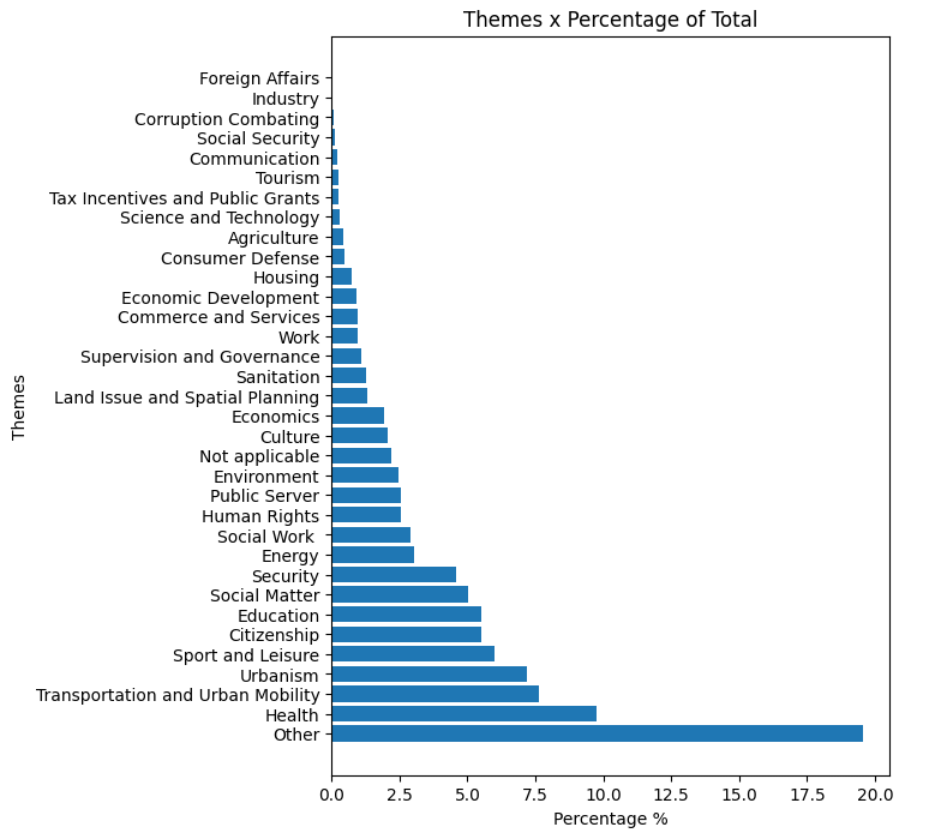
\includegraphics[width=0.8\textwidth]{fig/graphThemesPercentage.png}
	\caption{Themes x Percentage of Total}
	\label{fig:themes}
\end{figure}

This excessive reliance on the ``other'' category underscores significant deficiencies in the current classification system. It hinders effective tracking, analysis, and transparency of legislative activities, making it difficult for both the public and lawmakers to understand and manage the legislative process.


\section{Objectives}

This study aims to evaluate various machine learning models to determine which is most effective in suggesting more accurate thematic categories for legislative propositions. The goal is to identify themes that better align with the propositions, thus enhancing the relevance and accuracy of their categorization.

It is important to clarify that this study does not seek to automate the entire classification process, replace human classifiers, or compare human classification with machine learning-based methods. Instead, the focus is on improving the existing categorization process by identifying the best machine learning model for suggesting themes for propositions currently labeled as "Others."

\section{Methodology}

In the initial phase of the methodology, known as Business Understanding, we analyzed legislative documents to ensure our data mining objectives were aligned with the needs of legislative classification. This involved reviewing various legislative propositions and their metadata to align our goals with the requirements for effective classification.

The Data Understanding phase involved working with a dataset of 22,267 summaries extracted from the “Processo Legislativo Eletrônico (PLE)” system, covering the period from 2021 to May 2024. Each summary in this dataset is accompanied by its respective thematic classification, providing the foundation for further analysis.

Data Preparation included several critical steps. First, we discarded data classified under the “others” and “not applicable” categories. Following this, we performed preprocessing tasks such as tokenization, normalization, stopword removal, and lemmatization. For vectorization, we employed two techniques: the Multilingual Sentence Embedding Model, based on the MiniLM architecture, which generates high-quality embeddings capturing the semantic meaning of the text, and the TF-IDF (Term Frequency-Inverse Document Frequency) Model, which converts text into numerical vectors by evaluating term frequency within documents and across the dataset, thereby highlighting term importance.

In the Modeling phase, we utilized several models to address the classification task. The DummyClassifier was used as a baseline model to provide a reference point for comparing the performance of more complex models. The Support Vector Machine (SVM) was employed to find the hyperplane that best separates the classes in the feature space, proving effective in high-dimensional spaces. Logistic Regression, a linear model, was used to estimate the probability of a binary outcome based on input features, valued for its simplicity and interpretability. Additionally, XGBoost (Extreme Gradient Boosting) was chosen for its ability to build an ensemble of weak learners, such as decision trees, improving model performance through optimization. Random Forest, another ensemble model, constructs multiple decision trees and aggregates their predictions, demonstrating robustness against overfitting and effectiveness with larger datasets. Finally, K-Nearest Neighbors (KNN), a non-parametric model, classifies data points based on the majority class of their nearest neighbors, offering simplicity and effectiveness for smaller datasets.

The Evaluation phase focused on assessing model performance using various metrics. Accuracy was used as a straightforward measure of overall correctness. Precision and recall provided insights into performance, particularly with imbalanced classes, by focusing on the performance of minority classes. The F1 Score combined precision and recall into a single metric, summarizing model performance effectively.

Finally, in the Deployment phase, the results of the study could be used to create an interface within the “Processo Legislativo Eletrônico (PLE)” system. This interface would suggest themes that best fit new legislative propositions, thereby enhancing the legislative classification process.

\section{Experiments conducted}

In the experiments conducted, a cross-validation with three stratified partitions was performed for each model. The three partitions were randomly divided to allow for training and testing each model across all four metrics, both for training and testing data. Along with the four metrics, the training and inference times were also measured. For each metric, the average of the three validations was computed.

The primary aim of this approach was to assess overfitting and underfitting. Overfitting is indicated if there is good performance during training but poor performance during testing. Conversely, underfitting is suggested if there is poor performance in both training and testing phases.

For the embedding vectorizer experiments, Logistic Regression demonstrated overall excellence. Although it might not be the best in every individual metric, it consistently outperformed other models across the set of metrics.

Similarly, when using the Tfidf Vectorizer, Logistic Regression again emerged as the top performer. This model showed superior performance across the metrics compared to others.

In experiments involving the Tfidf Vectorizer combined with the MultiOutputClassifier, Logistic Regression continued to prove itself as the top-performing model. This combination did not alter the overall performance ranking of Logistic Regression, which remained the best-performing model across these experimental setups.

\section{Conclusions}

Logistic Regression, when trained with TfidfVectorizer and MultiOutputClassifier, achieved the best results. However, the analysis identified some accuracy issues. The classifications are not fully representative of the true distribution of legislative propositions, and the data volume is insufficient to meet desired objectives effectively.

Performance metrics indicated that:

\begin{itemize}
	\item The top 3 probabilities achieved an accuracy of 0.7027.
	\item The top 4 probabilities reached an accuracy of 0.7613.
	\item he top 5 probabilities resulted in an accuracy of 0.8030.
\end{itemize}

These results reflect the model's ability to suggest relevant categories based on the probabilities of different themes.

\section{Future work}


Future research should focus on integrating neural network models to explore their potential for improving classification accuracy. Additionally, refining class definitions and reclassifying the data will be essential to address current limitations and enhance the effectiveness of the classification process.

	
\bibliographystyle{sbc}
\bibliography{artigo}
	
\end{document}
